%---------- Quinto Capítulo: Resultados ----------

\chapter{Resultados} %5 --- 10 pags

Com o conjunto de ferramentas desenvolvidos neste projeto aliado a uma base de vídeos originais é possível produzir uma nova e diversificada base com vídeos degradados em qualidade e quantitade variável.
Neste Capítulo serão verificados os resultados obtidos a partir do processamento de vídeos efuados por estas ferramentas. Primeiramente uma avaliação subjetiva das ferramentas de degradação utilizando diversas amostras retiradas de um vídeo da base. A seguir é feita a validação dos resultados obtidos pela ferramenta de métricas objetivas, tomando como base (base do wyllian!!).
Por fim é feita uma análise das notas de avaliação objetivas buscando mensurar o impacto que determinadas degradações podem ter sobre um conjunto de vídeos com características diferentes.

\section{Validação das Ferramentas de Artefatos}

\begin{figure}[!htb]
	\centering
	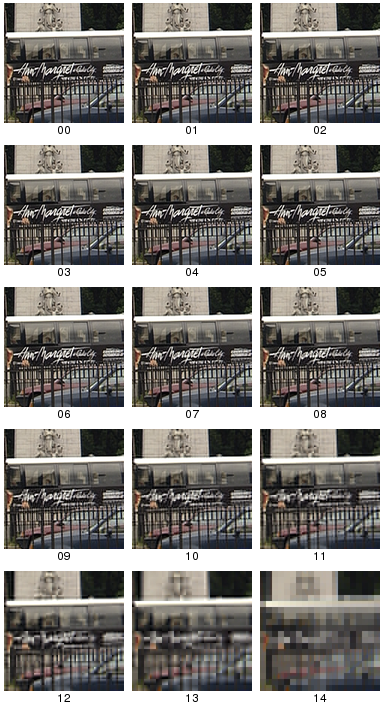
\includegraphics[width=0.9\textwidth]{./imgs/blockbus.png}
	\caption{.}
	\label{fig:blockbus}
	\fonte{Autoria Própria.}
\end{figure}

\begin{figure}[!htb]
	\centering
	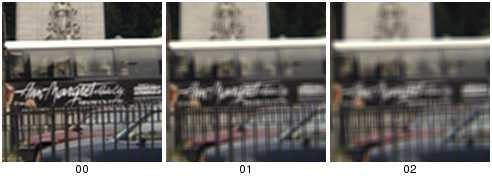
\includegraphics[width=0.9\textwidth]{./imgs/bluraverage.png}
	\caption{.}
	\label{fig:bluraverage}
	\fonte{Autoria Própria.}
\end{figure}

\begin{figure}[!htb]
	\centering
	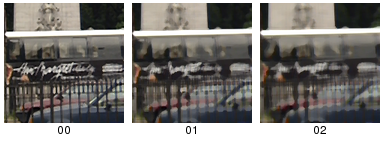
\includegraphics[width=0.9\textwidth]{./imgs/blurmedian.png}
	\caption{.}
	\label{fig:blurmedian}
	\fonte{Autoria Própria.}
\end{figure}

\begin{figure}[!htb]
	\centering
	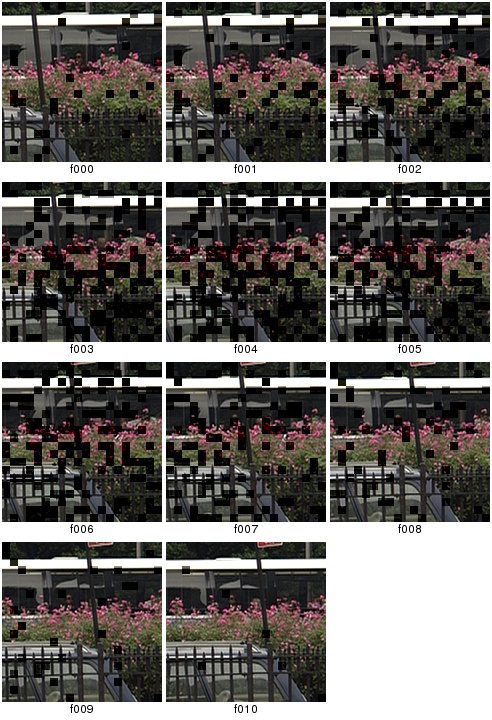
\includegraphics[width=0.7\textwidth]{./imgs/busraffle.png}
	\caption{.}
	\label{fig:busraffle}
	\fonte{Autoria Própria.}
\end{figure}

\begin{figure}[!htb]
	\centering
	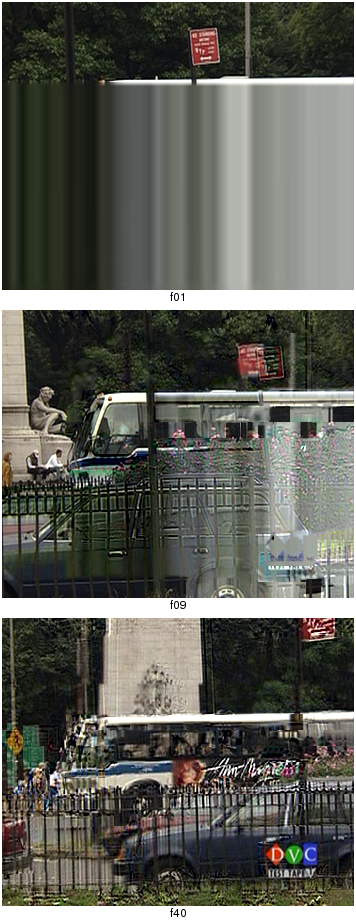
\includegraphics[height=0.9\textheight]{./imgs/netsimresult.png}
	\caption{.}
	\label{fig:netsim}
	\fonte{Autoria Própria.}
\end{figure}

\section{Validação da Ferramenta de Métricas}

\section{Análise de Impacto Sobre Métricas Objetivas}

\section{Resumo e Conclusão do Capítulo}
